\begin{question}[ID=xavyvn,type=exam]{10}
请考虑课堂上的餐厅博弈,其中Xavier和Yvonne的餐厅争夺顾客,Xavier的销售量由 $Q_x = 44 - 2P_x + P_y$ 给出,Yvonne的销售量由 $Q_y = 44 - 2P_y + P_x$ 给出,其中Xavier设定价格 $P_x$,Yvonne设定价格 $P_y$。\\
但现在他们的成本不再相同,假设Yvonne的每餐成本降低至 \vary{\$2}{\$4},而Xavier的每餐成本增加至 \vary{\$8}{\$12}。\\
Xavier的最优响应规则为:
$$ BR_x(P_y) = \frac{1}{4} P_y + \vary{15}{17} $$
Yvonne的最优响应规则为:
$$ BR_y(P_x) = \frac{1}{4} P_x + \vary{12}{13} $$
\begin{tasks}
  \task 
  求解该定价博弈中的所有纳什均衡。
  解释为何这些均衡是稳定的。
  \PrintSolutionsTF{
  \fbox{
    \parbox{\linewidth}{
    解:
    \vary
    {
    \begin{center}
    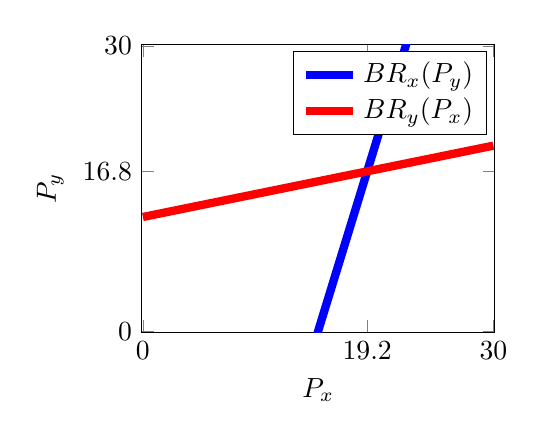
\begin{tikzpicture}
      \begin{axis}[
        width=.5\textwidth,
        xlabel={$P_x$},
        ylabel={$P_y$},
        xmin=-0.1, xmax=30.1,
        ymin=-0.1, ymax=30.1,
        xtick={0,19.2,30},
        ytick={0,16.8,30},
        ]
        \addplot [
        domain=0:30,
        line width=3pt,
        color=blue,
        ] 
        {4*x - 44 - 2*8};
        \addlegendentry{\(BR_x(P_y)\)}
        \addplot [
        domain=0:30,
        line width=3pt,
        color=red,
        ] 
        {11 + .5*2 + .25*x};
        \addlegendentry{\(BR_y(P_x)\)}
      \end{axis}
    \end{tikzpicture}
    \end{center}
    }
    {
    \begin{center}
    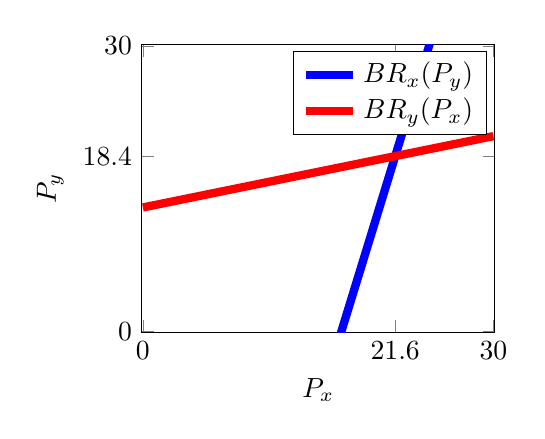
\begin{tikzpicture}
      \begin{axis}[
        width=.5\textwidth,
        xlabel={$P_x$},
        ylabel={$P_y$},
        xmin=-0.1, xmax=30.1,
        ymin=-0.1, ymax=30.1,
        xtick={0,21.6,30},
        ytick={0,18.4,30},
        ]
        \addplot [
        domain=0:30,
        line width=3pt,
        color=blue,
        ] 
        {4*x - 44 - 2*12};
        \addlegendentry{\(BR_x(P_y)\)}
        \addplot [
        domain=0:30,
        line width=3pt,
        color=red,
        ] 
        {11 + .5*4 + .25*x};
        \addlegendentry{\(BR_y(P_x)\)}
      \end{axis}
    \end{tikzpicture}
    \end{center}
    }
    在纳什均衡中,$BR_x(P_y) = P_x$ 且 $BR_y(P_x) = P_y$。
    \begin{align*}
      P_x & = \frac{1}{4}(\frac{1}{4}P_x + \vary{12}{13}) + \vary{15}{17} \\
      P_x & = \frac{1}{16}P_x + \frac{\vary{12}{13}}{4} + \vary{15}{17} \\
      \frac{15}{16} P_x & = \vary{18}{20.25} \\
      P_x^* & = \vary{19.2}{21.6}
    \end{align*}
    将 $P_x^*$ 代入 $BR_y()$:
    \begin{align*}
      P_y & = \frac{1}{4} (\vary{19.2}{21.6}) + \vary{12}{13} \\
      P_y^* & = \vary{16.8}{18.4}
    \end{align*}
    ($P_x =$ \vary{19.2}{21.6}, $P_y = $ \vary{16.8}{18.4})
    是游戏中唯一的纳什均衡,因为这是唯一一组使双方最优响应曲线相交的价格组合。
    }}
  }{
    \vspace{5cm}
  }
\end{tasks}
\end{question}

\begin{question}[ID=vlccs,type=exam]
原油通过名为超大型原油运输船(VLCCs)的巨型油轮在全球运输。
% 截至2001年,超过92%的新VLCC在南韩和日本建造。
假设新VLCC的价格(单位:百万美元)由函数 $P = 166 - Q$ 决定,
其中 $Q = q_{Korea} + q_{Japan}$。
(即假定仅日本和韩国生产VLCC,形成双寡头垄断。)
假设韩国每艘船的建造成本为\$\vary{7}{9}百万,日本为\$\vary{10}{14}百万。
即 $c_{Korea} = \vary{7}{9}$,$c_{Japan} = \vary{10}{14}$,
单船成本单位为百万美元。
\begin{tasks}
  \task (\points{4}) 求解韩国对日本产量的最优响应规则。
  \task (\points{4}) 求解日本对韩国产量的最优响应规则。
  \task (\points{4}) 以韩国产量为横轴、日本产量为纵轴,绘制最优响应曲线。
  \task (\points{4}) 求解所有纳什均衡。解释为何它们是稳定的。
\end{tasks}
\begin{solution}
  \begin{tasks}
    \task $BR_{Korea}(q_{Japan}) = \frac{166-q_{Japan}-\vary{7}{9}}{2} = \vary{78}{76}-0.5q_{Japan}$
    \par\noindent\rule{\linewidth}{0.4pt}
    答案正确得4分;步骤显示正确设定但存在代数错误得3分;答案错误且缺少步骤或设定错误得2分;答案错误且无步骤/证明得1分。
    \task $BR_{Japan}(q_{Korea}) = \frac{166-q_{Korea}-\vary{10}{14}}{2} = \vary{79.5}{78.5}-0.5q_{Korea}$
    \task 图像: \\
    \vary{
    \begin{center}
    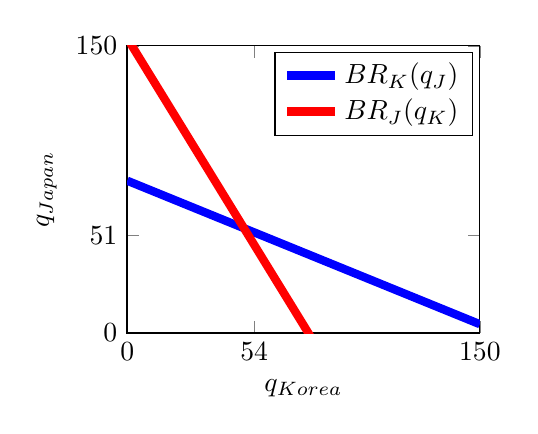
\begin{tikzpicture}
      \begin{axis}[
        width=.5\textwidth,
        xlabel={$q_{Korea}$},
        ylabel={$q_{Japan}$},
        xmin=-0.1, xmax=150,
        ymin=-0.1, ymax=150,
        xtick={0,54,150},
        ytick={0,51,150},
        ]
        \addplot [
        domain=0:150,
        line width=3pt,
        color=blue,
        ] 
        {79.5-0.5*x};
        \addlegendentry{\(BR_K(q_J)\)}
        \addplot [
        domain=0:150,
        line width=3pt,
        color=red,
        ] 
        {154-2*x};
        \addlegendentry{\(BR_J(q_K)\)}
      \end{axis}
    \end{tikzpicture}
    \end{center} 
    }{
    \begin{center}
    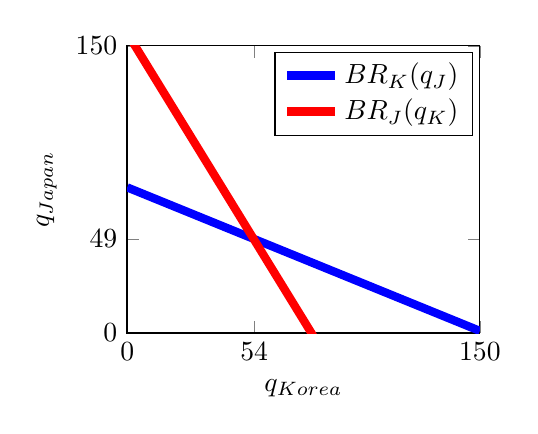
\begin{tikzpicture}
      \begin{axis}[
        width=.5\textwidth,
        xlabel={$q_{Korea}$},
        ylabel={$q_{Japan}$},
        xmin=-0.1, xmax=150,
        ymin=-0.1, ymax=150,
        xtick={0,54,150},
        ytick={0,49,150},
        ]
        \addplot [
        domain=0:150,
        line width=3pt,
        color=blue,
        ] 
        {76-0.5*x};
        \addlegendentry{\(BR_K(q_J)\)}
        \addplot [
        domain=0:150,
        line width=3pt,
        color=red,
        ] 
        {156.6-2*x};
        \addlegendentry{\(BR_J(q_K)\)}
      \end{axis}
    \end{tikzpicture}
    \end{center} 
    }
    \par\noindent\rule{\linewidth}{0.4pt}
    图像符合标准得4分;存在错误但与之前步骤一致或明显为次要错误得3分;错误但标注合理且符合学生步骤得2分;未标注且与步骤关联不清得1分。
  \task
    唯一纳什均衡为 ${q_K = \vary{54}{54}, q_J =  \vary{51}{49}}$
    这些数量是稳定的,例如若韩国降低价格,其利润将减少。
    同理适用于日本。
    \par\noindent\rule{\linewidth}{0.4pt}
    数值正确且解释合理得4分;数值有偏差但符合之前步骤且解释合理得3分;数值错误且不符合先前步骤或无合理解释得2分;答案错误且无步骤/解释得1分。
  \end{tasks}
\end{solution}
\end{question}
